

\begin{figure}
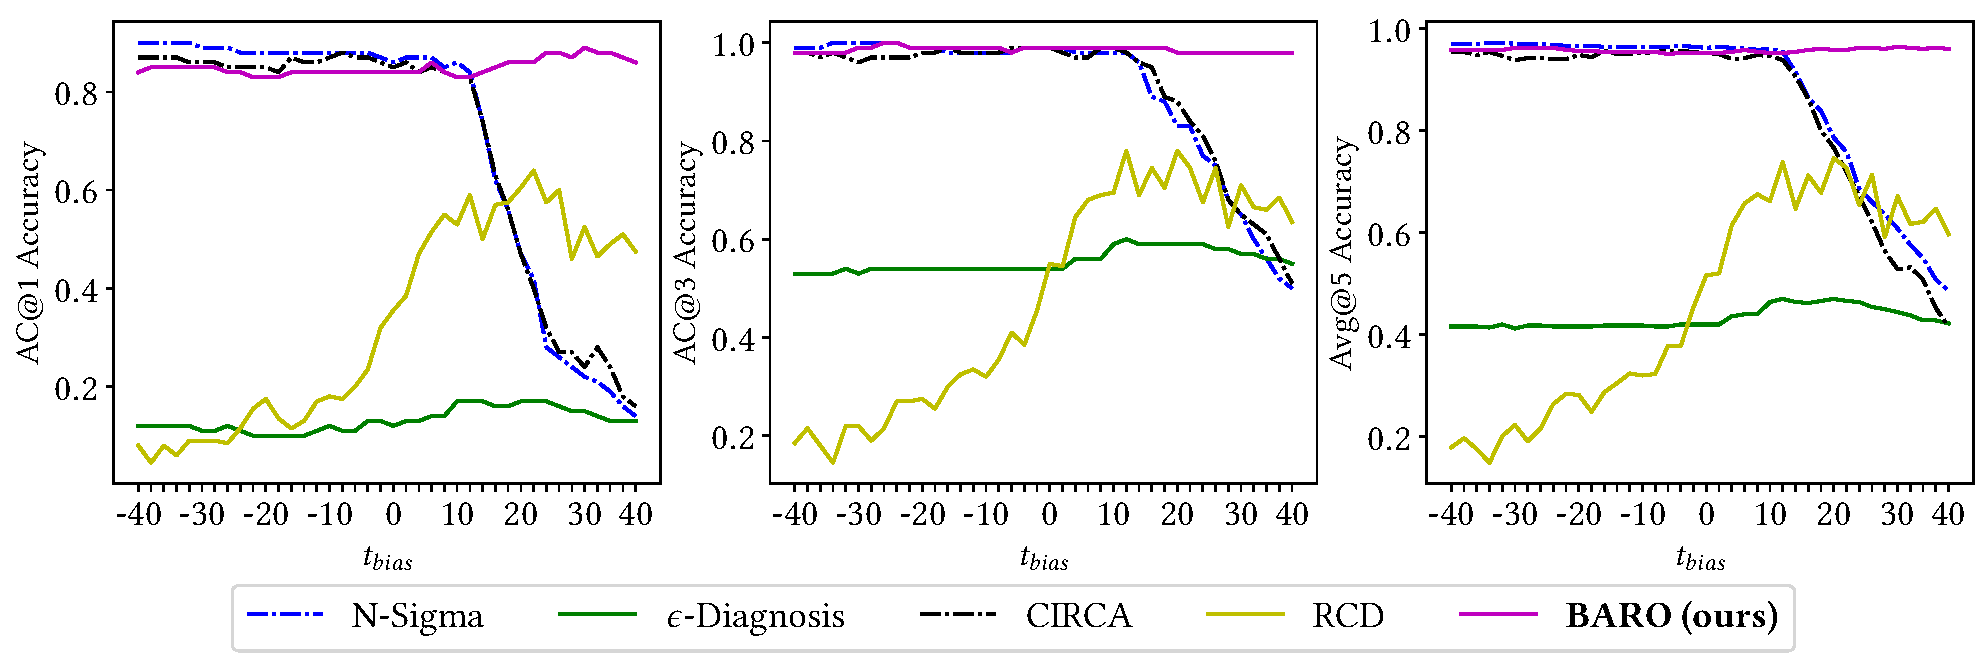
\includegraphics[width=0.9\textwidth]{image/q4-sensitivity-fse-ss.pdf}
\caption{AC@1, AC@3, and Avg@5 accuracy on the Sock Shop dataset w.r.t different $t_{bias}$. \hh{can make the figure shorter to save space}} \label{fig:q4-sensitivity-1}
\end{figure}




the list to check SLO checks
\begin{itemize}
    \item Eadro: NO
    \item CMdiagnotor: YES there is
    \item AdSketch: NO
    \item cIRCA: YES
    \item causalrca: no
    \item e-diagosis: YES
    \item RCD: no
    \item MicroScope: YES
    \item MsRank: NO
    \item Causeinfer: YES
    \item Microrca: YES
    \item microdiag: YES
\end{itemize}

CONCLUSION: WE NEED TO INCLUDE, hix

how other paper describe about the SLO 

\textbf{CMdiagnostor}; in their problem statement section, SLO: Service Level Objectives (SLOs) are adopted by the system we studied to measure customer satisfaction [1]. Once SLOs are violated, alerts covering information, such as alerting services, will generated to notify the operator.... the main objective of our paper is \textbf{once the system alerts for SLO violation is reported, we need to identify the most possible cause services as soon as possible based on previously collected method-level call metric data}. they do not describe SLO in introduction section. they do not have the background section. they had a terminology section to decribe about some basic terminilogy.

\textbf{CIRCA}: several metrics are the measures of the overall system health status, named the \textit{service level indicators} (SLIs) e.g. the average response time of an online sevice. Once an SLI violates the pre-defined service level objective (i.e. a failure occurs), operators will mitigate the failure as soon as possible to prevent further damage. as a single fault may propagate in the sstem s with multiple metrics eing abormal during a failure (anomay storm), RCA of the underlygiing fault can save much time for failure mitigation.

\textbf{e-diagnosis}: web services typically have strict SLO, tail latency, rather than average latency. however, diagosing SLI violation is a non trivial for large-scale web applications in shared microservice platforms due to million level operational data and complex operational exvironments.t

\textbf{MicroScope}: Microscope mainly collects two types of data: network connection information between two service instances and SLO (Service Level Objective) metrics of each service instance. To diagnose system anomalies, Microscope continually monitors the SLO metrics of the front end within a sliding time window. When an SLO violation is detected, the root cause analysis is triggered. In service causality graph building phase, Microscope uses the network connection information and SLO metrics to build a causality graph. 

\textbf{SLO (Service Level Objective) Metrics.} This type of data is used for detecting whether a service instance is abnormal and ranking root cause candidates. According to our observations, most cloud-native applications that internally generates performance metrics such as throughput for monitoring and maintenance. If these data are not internally available, we can also crawl the service logs to that end. For example, the spring boot framework provides a plug-in of service log for monitoring. Therefore, we can easily get SLO metrics from cloud-native applications in microservice environments. In this paper, we will use a unified SLO metric, namely service request latency which is the service calling time, which exposed by the services themselves. In the future work, we will explore more SLO metrics in microscope for improving the effectiveness. Although it is simple, it works well in Microscope.


If a value of SLO metric is not within the three-sigma interval of the last 10 min, we think this service instance is abnormal.

\textbf{causeinfer}: Once an SLO (Service Level Objective) violation in the front end servers occurs, the inference procedure is triggered. We first locate the performance anomaly at specific service(s) (e.g. tomcat) by detecting the violations of SLO metric then
find out the root cause(s) by detecting the violations of other performance metrics in a local node To further strengthen the robustness of the diagnosis we introduce a new change point detection method based on Bayesian theory

The inference is triggered by an SLO violation in the front end then iteratively goes to the back end services along the paths in the service dependency graph. If an SLO violation is detected in one node, the fine-grained


\textbf{MicroRCA}: In this paper, we propose a new system, MicroRCA, to locate root causes of performance issues in microservices. MicroRCA is an application-agnostic system designed for container-based microservices environments. It collects application and system levels metrics continuously and detects anomaly on SLO (Service Level Objective) metrics. Once an anomaly is detected, MicroRCA constructs an attributed graph with services and hosts to model the anomaly propagation among services. This graph does not only include the service call paths but also include services collocated on the same (virtual) machines. MicroRCA correlates anomaly symptoms of communicating services with relevant resource utilization to infer the potential abnormal services and ranks the potential root causes.

\textbf{microdiag}: In this paper, we propose an application-agnostic system named MicroDiag (Section IV) for real-time performance diagnosis in microservice systems without requiring any historical anomaly data. MicroDiag continuously collects metrics from components and detects anomalies on SLO (Service Level Objective) metrics. Once an anomaly is detected, MicroDiag infers fine-grained root causes by modeling the anomaly propagation with a metrics causality graph and ranking the culprit metrics by traversing along this graph. The metrics causality graph is derived from a component dependency graph with two causal inference methods, which are employed to detect anomaly propagation paths from diverse anomaly symptoms. As the metrics causality graph is based on causal inference between inter-dependent components, MicroDiag can easily scale to the number of components in the system. 






\begin{table}[]
\centering
\caption{RCA OB Coarse All}
\label{tab:rca-ob-coarse-all}
\resizebox{\textwidth}{!}{%
\setlength\tabcolsep{2pt}
\begin{tabular}{l|rrrr|rrrr|rrrr|rrrr|rrrr}
\hline
 & \multicolumn{4}{c|}{\textbf{CPU}} & \multicolumn{4}{c|}{\textbf{MEM}} & \multicolumn{4}{c|}{\textbf{DELAY}} & \multicolumn{4}{c|}{\textbf{LOSS}} & \multicolumn{4}{c}{\textbf{AVG}} \\ \cline{2-21} 
Method & \multicolumn{1}{c}{\textit{TOP1}} & \multicolumn{1}{c}{\textit{TOP3}} & \multicolumn{1}{c}{\textit{TOP5}} & \multicolumn{1}{c|}{\textit{A@5}} & \multicolumn{1}{c}{\textit{TOP1}} & \multicolumn{1}{c}{\textit{TOP3}} & \multicolumn{1}{c}{\textit{TOP5}} & \multicolumn{1}{c|}{\textit{A@5}} & \multicolumn{1}{c}{\textit{TOP1}} & \multicolumn{1}{c}{\textit{TOP3}} & \multicolumn{1}{c}{\textit{TOP5}} & \multicolumn{1}{c|}{\textit{A@5}} & \multicolumn{1}{c}{\textit{TOP1}} & \multicolumn{1}{c}{\textit{TOP3}} & \multicolumn{1}{c}{\textit{TOP5}} & \multicolumn{1}{c|}{\textit{A@5}} & \multicolumn{1}{c}{\textit{TOP1}} & \multicolumn{1}{c}{\textit{TOP3}} & \multicolumn{1}{c}{\textit{TOP5}} & \multicolumn{1}{c}{\textit{A@5}} \\ \hline
Dummy & 0.09 & 0.24 & 0.41 & 0.24 & 0.09 & 0.24 & 0.45 & 0.26 & 0.1 & 0.26 & 0.45 & 0.27 & 0.08 & 0.25 & 0.4 & 0.24 & 0.09 & 0.25 & 0.43 & 0.25 \\ \hline
CausalRCA & 0.58 & 0.91 & 0.96 & 0.85 & 0.74 & 0.94 & 0.98 & 0.91 & 0.66 & 0.91 & 0.98 & 0.86 & 0.31 & 0.61 & 0.76 & 0.58 & 0.57 & 0.84 & 0.92 & 0.8 \\ \hline
$\epsilon$-Diagnosis {[}delay 0{]} & 0 & 0.16 & 0.16 & 0.1 & 0 & 0.16 & 0.16 & 0.13 & 0 & 0.16 & 0.16 & 0.12 & 0.04 & 0.16 & 0.16 & 0.12 & 0.01 & 0.16 & 0.16 & 0.12 \\ \hline
$\epsilon$-Diagnosis {[}NSigma{]} & 0.04 & 0.24 & 0.24 & 0.19 & 0.08 & 0.2 & 0.2 & 0.16 & 0.08 & 0.28 & 0.28 & 0.23 & 0.08 & 0.28 & 0.28 & 0.22 & 0.07 & 0.25 & 0.25 & 0.2 \\ \hline
$\epsilon$-Diagnosis {[}BIRCH{]} & 0.16 & 0.36 & 0.36 & 0.31 & 0.04 & 0.29 & 0.29 & 0.23 & 0.12 & 0.24 & 0.24 & 0.2 & 0.12 & 0.2 & 0.2 & 0.18 & 0.11 & 0.27 & 0.27 & 0.23 \\ \hline
$\epsilon$-Diagnosis {[}SPOT{]} & 0.08 & 0.48 & 0.48 & 0.37 & 0.08 & 0.24 & 0.24 & 0.2 & 0.08 & 0.2 & 0.2 & 0.17 & 0.08 & 0.28 & 0.28 & 0.22 & 0.08 & 0.3 & 0.3 & 0.24 \\ \hline
$\epsilon$-Diagnosis {[}UniBCP{]} & 0.17 & 0.33 & 0.33 & 0.28 & 0 & 0.11 & 0.11 & 0.09 & 0.17 & 0.5 & 0.5 & 0.4 & 0 & 0.29 & 0.29 & 0.2 & 0.07 & 0.3 & 0.3 & 0.23 \\ \hline
$\epsilon$-Diagnosis {[}BOCPD{]} & 0.12 & 0.28 & 0.28 & 0.23 & 0.04 & 0.12 & 0.12 & 0.09 & 0 & 0.24 & 0.24 & 0.18 & 0 & 0.2 & 0.2 & 0.15 & 0.04 & 0.21 & 0.21 & 0.16 \\ \hline
RCD {[}delay 0{]} & 0.61 & 0.71 & 0.74 & 0.69 & 0.34 & 0.41 & 0.46 & 0.4 & 0.2 & 0.26 & 0.34 & 0.27 & 0.29 & 0.52 & 0.72 & 0.5 & 0.36 & 0.48 & 0.57 & 0.46 \\ \hline
RCD {[}NSigma{]} & 0.58 & 0.65 & 0.75 & 0.67 & 0.35 & 0.44 & 0.51 & 0.43 & 0.2 & 0.31 & 0.41 & 0.31 & 0.25 & 0.5 & 0.71 & 0.49 & 0.34 & 0.48 & 0.6 & 0.48 \\ \hline
RCD {[}BIRCH{]} & 0.55 & 0.67 & 0.74 & 0.65 & 0.34 & 0.4 & 0.43 & 0.39 & 0.22 & 0.28 & 0.34 & 0.29 & 0.32 & 0.47 & 0.66 & 0.49 & 0.36 & 0.46 & 0.55 & 0.46 \\ \hline
RCD {[}SPOT{]} & 0.62 & 0.7 & 0.76 & 0.7 & 0.34 & 0.41 & 0.51 & 0.42 & 0.22 & 0.29 & 0.37 & 0.3 & 0.28 & 0.5 & 0.64 & 0.48 & 0.36 & 0.47 & 0.57 & 0.47 \\ \hline
RCD {[}UniBCP{]} & 0.57 & 0.67 & 0.73 & 0.66 & 0.35 & 0.42 & 0.51 & 0.42 & 0.21 & 0.3 & 0.36 & 0.29 & 0.24 & 0.52 & 0.73 & 0.49 & 0.34 & 0.48 & 0.58 & 0.47 \\ \hline
RCD {[}BOCPD{]} & 0.59 & 0.7 & 0.77 & 0.7 & 0.32 & 0.41 & 0.46 & 0.4 & 0.24 & 0.32 & 0.34 & 0.3 & 0.32 & 0.53 & 0.67 & 0.52 & 0.37 & 0.49 & 0.56 & 0.48 \\ \hline
CIRCA {[}delay 0{]} & 0.56 & 1 & 1 & 0.9 & 0.6 & 0.8 & 0.8 & 0.74 & 0.72 & 0.96 & 0.96 & 0.9 & 0.4 & 0.6 & 0.6 & 0.55 & 0.57 & 0.84 & 0.84 & 0.77 \\ \hline
CIRCA {[}NSigma{]} & 0.4 & 0.88 & 0.88 & 0.78 & 0.4 & 0.68 & 0.68 & 0.59 & 0.6 & 0.84 & 0.84 & 0.79 & 0.36 & 0.52 & 0.52 & 0.48 & 0.44 & 0.73 & 0.73 & 0.66 \\ \hline
CIRCA {[}BIRCH{]} & 0.33 & 0.67 & 0.67 & 0.57 & 0.17 & 0.42 & 0.42 & 0.35 & 0.24 & 0.36 & 0.36 & 0.34 & 0.17 & 0.21 & 0.21 & 0.19 & 0.22 & 0.4 & 0.4 & 0.36 \\ \hline
CIRCA {[}SPOT{]} & 0.48 & 0.84 & 0.84 & 0.76 & 0.52 & 0.76 & 0.76 & 0.7 & 0.64 & 0.96 & 0.96 & 0.88 & 0.56 & 0.68 & 0.68 & 0.66 & 0.55 & 0.81 & 0.81 & 0.75 \\ \hline
CIRCA {[}UniBCP{]} & 0 & 0.2 & 0.2 & 0.16 & 0 & 0 & 0 & 0 & 0 & 0 & 0 & 0 & 0.08 & 0.5 & 0.5 & 0.35 & 0.05 & 0.35 & 0.35 & 0.25 \\ \hline
CIRCA {[}BOCPD{]} & 0.44 & 0.76 & 0.76 & 0.68 & 0.12 & 0.24 & 0.24 & 0.2 & 0.16 & 0.32 & 0.32 & 0.28 & 0.24 & 0.48 & 0.48 & 0.42 & 0.24 & 0.45 & 0.45 & 0.39 \\ \hline
NSigma {[}delay 0{]} & 0.52 & 1 & 1 & 0.9 & 0.68 & 1 & 1 & 0.93 & 0.72 & 1 & 1 & 0.94 & 0.44 & 0.68 & 0.88 & 0.66 & 0.59 & 0.92 & 0.97 & 0.85 \\ \hline
NSigma {[}NSigma{]} & 0.44 & 0.88 & 0.92 & 0.79 & 0.52 & 0.72 & 0.8 & 0.69 & 0.64 & 0.88 & 0.88 & 0.83 & 0.4 & 0.64 & 0.88 & 0.63 & 0.5 & 0.78 & 0.87 & 0.74 \\ \hline
NSigma {[}BIRCH{]} & 0.2 & 0.6 & 0.68 & 0.53 & 0.21 & 0.42 & 0.63 & 0.43 & 0.32 & 0.56 & 0.6 & 0.51 & 0.08 & 0.48 & 0.64 & 0.39 & 0.2 & 0.52 & 0.64 & 0.47 \\ \hline
NSigma {[}SPOT{]} & 0.48 & 0.88 & 0.92 & 0.79 & 0.6 & 0.84 & 0.88 & 0.79 & 0.72 & 1 & 1 & 0.93 & 0.48 & 0.64 & 0.84 & 0.65 & 0.57 & 0.84 & 0.91 & 0.79 \\ \hline
NSigma {[}UniBCP{]} & 0.58 & 0.83 & 0.83 & 0.75 & 0.33 & 0.78 & 0.78 & 0.69 & 0.71 & 1 & 1 & 0.91 & 0.53 & 0.82 & 0.94 & 0.76 & 0.53 & 0.84 & 0.89 & 0.77 \\ \hline
NSigma {[}BOCPD{]} & 0.4 & 0.76 & 0.96 & 0.74 & 0.08 & 0.28 & 0.6 & 0.32 & 0.32 & 0.52 & 0.68 & 0.52 & 0.36 & 0.56 & 0.8 & 0.58 & 0.29 & 0.53 & 0.76 & 0.54 \\ \hline
PC + RS {[}delay 0{]} & 0.44 & 0.88 & 0.88 & 0.76 & 0.6 & 0.88 & 0.88 & 0.78 & 0.56 & 0.96 & 0.96 & 0.84 & 0.28 & 0.52 & 0.52 & 0.46 & 0.47 & 0.81 & 0.81 & 0.71 \\ \hline
PC + RS {[}N-Sigma{]} & 0.4 & 0.92 & 0.92 & 0.79 & 0.48 & 0.68 & 0.68 & 0.62 & 0.44 & 0.84 & 0.84 & 0.74 & 0.24 & 0.48 & 0.48 & 0.42 & 0.39 & 0.73 & 0.73 & 0.64 \\ \hline
PC + RS {[}BIRCH{]} & 0.19 & 0.57 & 0.57 & 0.46 & 0.25 & 0.42 & 0.42 & 0.38 & 0.2 & 0.28 & 0.28 & 0.26 & 0.04 & 0.21 & 0.21 & 0.17 & 0.17 & 0.36 & 0.36 & 0.31 \\ \hline
PC + RS {[}SPOT{]} & 0.44 & 0.8 & 0.8 & 0.67 & 0.6 & 0.88 & 0.88 & 0.81 & 0.48 & 0.92 & 0.92 & 0.82 & 0.36 & 0.76 & 0.76 & 0.66 & 0.47 & 0.84 & 0.84 & 0.74 \\ \hline
PC + RS {[}UniBCP{]} & 0.2 & 0.4 & 0.4 & 0.32 & 0 & 0 & 0 & 0 & 0 & 0 & 0 & 0 & 0.17 & 0.5 & 0.5 & 0.4 & 0.15 & 0.4 & 0.4 & 0.32 \\ \hline
PC + RS {[}BOCPD{]} & 0.32 & 0.68 & 0.68 & 0.57 & 0.24 & 0.48 & 0.48 & 0.4 & 0.08 & 0.6 & 0.6 & 0.49 & 0.24 & 0.44 & 0.44 & 0.38 & 0.22 & 0.55 & 0.55 & 0.46 \\ \hline
\textit{RobustScorer {[}delay 0{]}} & 0.6 & 1 & 1 & 0.9 & 0.76 & 1 & 1 & 0.94 & 0.68 & 1 & 1 & 0.94 & 0.44 & 0.6 & 0.92 & 0.65 & 0.62 & 0.9 & 0.98 & 0.86 \\ \hline
\textit{RobustScorer {[}NSigma{]}} & 0.6 & 1 & 1 & 0.9 & 0.84 & 1 & 1 & 0.96 & 0.72 & 0.92 & 0.92 & 0.88 & 0.4 & 0.64 & 0.76 & 0.58 & 0.64 & 0.89 & 0.92 & 0.83 \\ \hline
\textit{RobustScorer {[}BIRCH{]}} & 0.36 & 0.72 & 0.76 & 0.65 & 0.5 & 0.75 & 0.83 & 0.72 & 0.4 & 0.68 & 0.68 & 0.62 & 0.2 & 0.4 & 0.68 & 0.44 & 0.36 & 0.64 & 0.74 & 0.6 \\ \hline
\textit{RobustScorer {[}SPOT{]}} & 0.56 & 1 & 1 & 0.89 & 0.76 & 1 & 1 & 0.94 & 0.68 & 1 & 1 & 0.93 & 0.44 & 0.64 & 0.76 & 0.61 & 0.61 & 0.91 & 0.94 & 0.84 \\ \hline
\textit{RobustScorer {[}UniBCP{]}} & 0.5 & 0.83 & 0.83 & 0.73 & 0.33 & 0.67 & 0.89 & 0.67 & 0.71 & 1 & 1 & 0.89 & 0.47 & 0.88 & 0.94 & 0.79 & 0.49 & 0.84 & 0.91 & 0.76 \\ \hline
\textit{\textbf{\begin{tabular}[c]{@{}l@{}}RobustScorer {[}BOCPD{]}\\ (Our BARO method)\end{tabular}}} & 0.64 & 1 & 1 & 0.91 & 0.8 & 1 & 1 & 0.96 & 0.76 & 1 & 1 & 0.95 & 0.44 & 0.6 & 0.88 & 0.62 & 0.66 & 0.9 & 0.97 & 0.86 \\ \hline
\end{tabular}%
}
\end{table}



\begin{table}[]
\centering
\caption{RCA SS Coarse All}
\label{tab:rca-ss-coarse-all}
\resizebox{\textwidth}{!}{%
\setlength\tabcolsep{2pt}
\begin{tabular}{l|rrrr|rrrr|rrrr|rrrr|rrrr}
\hline
 & \multicolumn{4}{c|}{\textbf{CPU}} & \multicolumn{4}{c|}{\textbf{MEM}} & \multicolumn{4}{c|}{\textbf{DELAY}} & \multicolumn{4}{c|}{\textbf{LOSS}} & \multicolumn{4}{c}{\textbf{AVG}} \\ \cline{2-21} 
Method & \multicolumn{1}{c}{\textit{TOP1}} & \multicolumn{1}{c}{\textit{TOP3}} & \multicolumn{1}{c}{\textit{TOP5}} & \multicolumn{1}{c|}{\textit{A@5}} & \multicolumn{1}{c}{\textit{TOP1}} & \multicolumn{1}{c}{\textit{TOP3}} & \multicolumn{1}{c}{\textit{TOP5}} & \multicolumn{1}{c|}{\textit{A@5}} & \multicolumn{1}{c}{\textit{TOP1}} & \multicolumn{1}{c}{\textit{TOP3}} & \multicolumn{1}{c}{\textit{TOP5}} & \multicolumn{1}{c|}{\textit{A@5}} & \multicolumn{1}{c}{\textit{TOP1}} & \multicolumn{1}{c}{\textit{TOP3}} & \multicolumn{1}{c}{\textit{TOP5}} & \multicolumn{1}{c|}{\textit{A@5}} & \multicolumn{1}{c}{\textit{TOP1}} & \multicolumn{1}{c}{\textit{TOP3}} & \multicolumn{1}{c}{\textit{TOP5}} & \multicolumn{1}{c}{\textit{A@5}} \\ \hline
Dummy & 0.12 & 0.34 & 0.58 & 0.34 & 0.14 & 0.41 & 0.66 & 0.4 & 0.1 & 0.32 & 0.61 & 0.34 & 0.11 & 0.36 & 0.59 & 0.36 & 0.12 & 0.36 & 0.61 & 0.36 \\ \hline
CausalRCA & 0.22 & 0.56 & 0.65 & 0.49 & 0.37 & 0.97 & 0.99 & 0.82 & 0.24 & 0.7 & 0.83 & 0.61 & 0.21 & 0.48 & 0.66 & 0.47 & 0.26 & 0.68 & 0.78 & 0.6 \\ \hline
$\epsilon$-Diagnosis {[}delay 0{]} & 0.16 & 0.6 & 0.6 & 0.47 & 0 & 0.44 & 0.44 & 0.3 & 0.2 & 0.52 & 0.52 & 0.42 & 0.16 & 0.6 & 0.6 & 0.49 & 0.13 & 0.54 & 0.54 & 0.42 \\ \hline
$\epsilon$-Diagnosis {[}NSigma{]} & 0.24 & 0.6 & 0.6 & 0.49 & 0.08 & 0.56 & 0.56 & 0.39 & 0.16 & 0.6 & 0.6 & 0.46 & 0.12 & 0.6 & 0.6 & 0.5 & 0.15 & 0.59 & 0.59 & 0.46 \\ \hline
$\epsilon$-Diagnosis {[}BIRCH{]} & 0.13 & 0.58 & 0.58 & 0.44 & 0.17 & 0.58 & 0.58 & 0.44 & 0.21 & 0.63 & 0.63 & 0.52 & 0.2 & 0.48 & 0.48 & 0.41 & 0.18 & 0.57 & 0.57 & 0.45 \\ \hline
$\epsilon$-Diagnosis {[}SPOT{]} & 0.2 & 0.56 & 0.56 & 0.46 & 0 & 0.52 & 0.52 & 0.34 & 0.12 & 0.56 & 0.56 & 0.42 & 0.16 & 0.56 & 0.56 & 0.46 & 0.12 & 0.55 & 0.55 & 0.42 \\ \hline
$\epsilon$-Diagnosis {[}UniBCP{]} & 0.14 & 0.21 & 0.21 & 0.2 & 0.13 & 0.2 & 0.2 & 0.19 & 0.13 & 0.31 & 0.31 & 0.25 & 0.12 & 0.24 & 0.24 & 0.2 & 0.13 & 0.24 & 0.24 & 0.21 \\ \hline
$\epsilon$-Diagnosis {[}BOCPD{]} & 0.12 & 0.56 & 0.56 & 0.45 & 0 & 0.52 & 0.52 & 0.35 & 0.12 & 0.52 & 0.52 & 0.38 & 0.08 & 0.56 & 0.56 & 0.44 & 0.08 & 0.54 & 0.54 & 0.41 \\ \hline
RCD {[}delay 0{]} & 0.5 & 0.65 & 0.68 & 0.62 & 0.38 & 0.46 & 0.57 & 0.46 & 0.26 & 0.51 & 0.62 & 0.48 & 0.23 & 0.37 & 0.5 & 0.37 & 0.34 & 0.5 & 0.59 & 0.48 \\ \hline
RCD {[}NSigma{]} & 0.42 & 0.54 & 0.65 & 0.54 & 0.34 & 0.41 & 0.52 & 0.42 & 0.24 & 0.47 & 0.6 & 0.46 & 0.25 & 0.38 & 0.47 & 0.37 & 0.31 & 0.45 & 0.56 & 0.45 \\ \hline
RCD {[}BIRCH{]} & 0.45 & 0.55 & 0.63 & 0.55 & 0.35 & 0.46 & 0.54 & 0.45 & 0.28 & 0.47 & 0.58 & 0.45 & 0.25 & 0.4 & 0.45 & 0.38 & 0.33 & 0.47 & 0.55 & 0.46 \\ \hline
RCD {[}SPOT{]} & 0.46 & 0.58 & 0.69 & 0.58 & 0.33 & 0.46 & 0.55 & 0.43 & 0.26 & 0.47 & 0.62 & 0.46 & 0.26 & 0.36 & 0.41 & 0.34 & 0.32 & 0.47 & 0.57 & 0.46 \\ \hline
RCD {[}UniBCP{]} & 0.5 & 0.63 & 0.7 & 0.62 & 0.36 & 0.44 & 0.55 & 0.44 & 0.28 & 0.52 & 0.66 & 0.5 & 0.26 & 0.37 & 0.46 & 0.36 & 0.35 & 0.49 & 0.59 & 0.48 \\ \hline
RCD {[}BOCPD{]} & 0.5 & 0.6 & 0.69 & 0.6 & 0.36 & 0.49 & 0.56 & 0.47 & 0.29 & 0.5 & 0.62 & 0.48 & 0.24 & 0.36 & 0.46 & 0.36 & 0.35 & 0.49 & 0.58 & 0.48 \\ \hline
CIRCA {[}delay 0{]} & 0.88 & 1 & 1 & 0.97 & 0.92 & 1 & 1 & 0.98 & 0.92 & 1 & 1 & 0.98 & 0.72 & 0.96 & 0.96 & 0.88 & 0.86 & 0.99 & 0.99 & 0.95 \\ \hline
CIRCA {[}NSigma{]} & 0.8 & 0.88 & 0.88 & 0.86 & 0.64 & 0.72 & 0.72 & 0.7 & 0.72 & 0.92 & 0.92 & 0.87 & 0.6 & 0.76 & 0.76 & 0.7 & 0.69 & 0.82 & 0.82 & 0.78 \\ \hline
CIRCA {[}BIRCH{]} & 0.21 & 0.5 & 0.5 & 0.41 & 0.35 & 0.43 & 0.43 & 0.42 & 0.35 & 0.48 & 0.48 & 0.43 & 0.21 & 0.67 & 0.67 & 0.52 & 0.28 & 0.52 & 0.52 & 0.45 \\ \hline
CIRCA {[}SPOT{]} & 0.8 & 0.84 & 0.84 & 0.83 & 0.84 & 0.88 & 0.88 & 0.87 & 0.8 & 1 & 1 & 0.95 & 0.64 & 0.84 & 0.84 & 0.78 & 0.77 & 0.89 & 0.89 & 0.86 \\ \hline
CIRCA {[}UniBCP{]} & 0 & 0.38 & 0.38 & 0.23 & 0 & 0 & 0 & 0 & 0 & 0.25 & 0.25 & 0.2 & 0.09 & 0.45 & 0.45 & 0.36 & 0.04 & 0.39 & 0.39 & 0.29 \\ \hline
CIRCA {[}BOCPD{]} & 0.64 & 0.76 & 0.76 & 0.73 & 0.92 & 1 & 1 & 0.98 & 0.32 & 0.6 & 0.6 & 0.54 & 0.36 & 0.76 & 0.76 & 0.66 & 0.56 & 0.78 & 0.78 & 0.73 \\ \hline
NSigma {[}delay 0{]} & 0.92 & 1 & 1 & 0.98 & 0.92 & 1 & 1 & 0.98 & 0.92 & 1 & 1 & 0.98 & 0.68 & 0.96 & 1 & 0.9 & 0.86 & 0.99 & 1 & 0.96 \\ \hline
NSigma {[}NSigma{]} & 0.76 & 0.88 & 0.88 & 0.85 & 0.64 & 0.76 & 0.88 & 0.77 & 0.84 & 0.88 & 0.92 & 0.89 & 0.56 & 0.84 & 0.96 & 0.79 & 0.7 & 0.84 & 0.91 & 0.82 \\ \hline
NSigma {[}BIRCH{]} & 0.63 & 0.75 & 0.75 & 0.72 & 0.58 & 0.75 & 0.88 & 0.73 & 0.42 & 0.54 & 0.75 & 0.6 & 0.4 & 0.56 & 0.88 & 0.61 & 0.51 & 0.65 & 0.81 & 0.66 \\ \hline
NSigma {[}SPOT{]} & 0.8 & 0.88 & 0.92 & 0.87 & 0.84 & 0.88 & 1 & 0.91 & 0.96 & 1 & 1 & 0.99 & 0.6 & 0.84 & 0.96 & 0.82 & 0.8 & 0.9 & 0.97 & 0.9 \\ \hline
NSigma {[}UniBCP{]} & 0.86 & 0.86 & 0.86 & 0.86 & 0.67 & 0.73 & 0.93 & 0.79 & 0.59 & 0.71 & 0.76 & 0.69 & 0.61 & 0.78 & 1 & 0.81 & 0.67 & 0.77 & 0.89 & 0.78 \\ \hline
NSigma {[}BOCPD{]} & 0.56 & 0.84 & 0.96 & 0.8 & 0.92 & 1 & 1 & 0.98 & 0.36 & 0.72 & 0.8 & 0.63 & 0.28 & 0.6 & 0.88 & 0.62 & 0.53 & 0.79 & 0.91 & 0.76 \\ \hline
PC + RS {[}delay 0{]} & 0.72 & 0.96 & 0.96 & 0.88 & 0.92 & 1 & 1 & 0.98 & 0.92 & 1 & 1 & 0.98 & 0.6 & 0.92 & 0.92 & 0.83 & 0.79 & 0.97 & 0.97 & 0.92 \\ \hline
PC + RS {[}N-Sigma{]} & 0.76 & 0.88 & 0.88 & 0.85 & 0.8 & 0.96 & 0.96 & 0.93 & 0.72 & 0.92 & 0.92 & 0.87 & 0.56 & 0.72 & 0.72 & 0.68 & 0.71 & 0.87 & 0.87 & 0.83 \\ \hline
PC + RS {[}BIRCH{]} & 0.21 & 0.42 & 0.42 & 0.35 & 0.43 & 0.7 & 0.7 & 0.64 & 0.26 & 0.43 & 0.43 & 0.4 & 0.13 & 0.42 & 0.42 & 0.35 & 0.26 & 0.49 & 0.49 & 0.43 \\ \hline
PC + RS {[}SPOT{]} & 0.84 & 0.92 & 0.92 & 0.9 & 0.88 & 0.96 & 0.96 & 0.94 & 0.8 & 1 & 1 & 0.96 & 0.68 & 0.92 & 0.92 & 0.85 & 0.8 & 0.95 & 0.95 & 0.91 \\ \hline
PC + RS {[}UniBCP{]} & 0.13 & 0.38 & 0.38 & 0.3 & 0 & 0 & 0 & 0 & 0 & 0.25 & 0.25 & 0.2 & 0.18 & 0.27 & 0.27 & 0.24 & 0.13 & 0.3 & 0.3 & 0.25 \\ \hline
PC + RS {[}BOCPD{]} & 0.56 & 0.88 & 0.88 & 0.79 & 0.88 & 1 & 1 & 0.98 & 0.48 & 0.84 & 0.84 & 0.76 & 0.48 & 0.88 & 0.88 & 0.74 & 0.6 & 0.9 & 0.9 & 0.82 \\ \hline
\textit{RobustScorer {[}delay 0{]}} & 0.92 & 1 & 1 & 0.98 & 0.88 & 1 & 1 & 0.98 & 0.92 & 1 & 1 & 0.98 & 0.64 & 0.96 & 0.96 & 0.86 & 0.84 & 0.99 & 0.99 & 0.95 \\ \hline
\textit{RobustScorer {[}NSigma{]}} & 0.84 & 1 & 1 & 0.96 & 0.88 & 1 & 1 & 0.98 & 0.92 & 1 & 1 & 0.98 & 0.72 & 1 & 1 & 0.9 & 0.84 & 1 & 1 & 0.96 \\ \hline
\textit{RobustScorer {[}BIRCH{]}} & 0.71 & 0.83 & 0.83 & 0.8 & 0.75 & 0.88 & 0.96 & 0.87 & 0.5 & 0.75 & 0.88 & 0.73 & 0.44 & 0.76 & 0.88 & 0.7 & 0.6 & 0.8 & 0.89 & 0.77 \\ \hline
\textit{RobustScorer {[}SPOT{]}} & 0.88 & 1 & 1 & 0.97 & 0.92 & 1 & 1 & 0.98 & 0.96 & 1 & 1 & 0.99 & 0.64 & 0.92 & 1 & 0.86 & 0.85 & 0.98 & 1 & 0.95 \\ \hline
\textit{RobustScorer {[}UniBCP{]}} & 0.71 & 0.79 & 0.86 & 0.8 & 0.47 & 0.6 & 0.87 & 0.65 & 0.59 & 0.71 & 0.76 & 0.69 & 0.61 & 0.89 & 1 & 0.84 & 0.59 & 0.75 & 0.88 & 0.75 \\ \hline
\textit{\textbf{\begin{tabular}[c]{@{}l@{}}RobustScorer {[}BOCPD{]}\\ (Our BARO method)\end{tabular}}} & 0.88 & 1 & 1 & 0.97 & 0.88 & 1 & 1 & 0.98 & 0.92 & 1 & 1 & 0.98 & 0.64 & 0.92 & 1 & 0.87 & 0.83 & 0.98 & 1 & 0.95 \\ \hline
\end{tabular}%
}
\end{table}


\begin{table}[]
\centering
\caption{RCA TT Coarse All}
\label{tab:rca-tt-coarse-all}
\resizebox{\textwidth}{!}{%
\setlength\tabcolsep{2pt}
\begin{tabular}{l|rrrr|rrrr|rrrr|rrrr|rrrr}
\hline
 & \multicolumn{4}{c|}{\textbf{CPU}} & \multicolumn{4}{c|}{\textbf{MEM}} & \multicolumn{4}{c|}{\textbf{DELAY}} & \multicolumn{4}{c|}{\textbf{LOSS}} & \multicolumn{4}{c}{\textbf{AVG}} \\ \cline{2-21} 
Method & \multicolumn{1}{c}{\textit{TOP1}} & \multicolumn{1}{c}{\textit{TOP3}} & \multicolumn{1}{c}{\textit{TOP5}} & \multicolumn{1}{c|}{\textit{A@5}} & \multicolumn{1}{c}{\textit{TOP1}} & \multicolumn{1}{c}{\textit{TOP3}} & \multicolumn{1}{c}{\textit{TOP5}} & \multicolumn{1}{c|}{\textit{A@5}} & \multicolumn{1}{c}{\textit{TOP1}} & \multicolumn{1}{c}{\textit{TOP3}} & \multicolumn{1}{c}{\textit{TOP5}} & \multicolumn{1}{c|}{\textit{A@5}} & \multicolumn{1}{c}{\textit{TOP1}} & \multicolumn{1}{c}{\textit{TOP3}} & \multicolumn{1}{c}{\textit{TOP5}} & \multicolumn{1}{c|}{\textit{A@5}} & \multicolumn{1}{c}{\textit{TOP1}} & \multicolumn{1}{c}{\textit{TOP3}} & \multicolumn{1}{c}{\textit{TOP5}} & \multicolumn{1}{c}{\textit{A@5}} \\ \hline
Dummy & 0.02 & 0.07 & 0.11 & 0.07 & 0.03 & 0.08 & 0.12 & 0.08 & 0.02 & 0.08 & 0.11 & 0.07 & 0.03 & 0.07 & 0.12 & 0.07 & 0.02 & 0.07 & 0.11 & 0.07 \\ \hline
CausalRCA & 0.3 & 0.58 & 0.7 & 0.53 & 0.11 & 0.31 & 0.5 & 0.3 & 0.08 & 0.17 & 0.26 & 0.17 & 0.02 & 0.12 & 0.18 & 0.11 & 0.13 & 0.3 & 0.41 & 0.28 \\ \hline
$\epsilon$-Diagnosis {[}delay 0{]} & 0 & 0 & 0 & 0 & 0 & 0.04 & 0.04 & 0.02 & 0 & 0 & 0 & 0 & 0 & 0 & 0 & 0 & 0 & 0.01 & 0.01 & 0.01 \\ \hline
$\epsilon$-Diagnosis {[}NSigma{]} & 0 & 0 & 0 & 0 & 0 & 0 & 0 & 0 & 0 & 0 & 0 & 0 & 0 & 0.04 & 0.04 & 0.02 & 0 & 0.01 & 0.01 & 0.01 \\ \hline
$\epsilon$-Diagnosis {[}BIRCH{]} & 0 & 0 & 0 & 0 & 0 & 0 & 0 & 0 & 0 & 0 & 0 & 0 & 0 & 0.08 & 0.08 & 0.06 & 0 & 0.02 & 0.02 & 0.01 \\ \hline
$\epsilon$-Diagnosis {[}SPOT{]} & 0 & 0 & 0 & 0 & 0 & 0.04 & 0.04 & 0.02 & 0 & 0 & 0 & 0 & 0 & 0 & 0 & 0 & 0 & 0.01 & 0.01 & 0.01 \\ \hline
$\epsilon$-Diagnosis {[}UniBCP{]} & 0 & 0.08 & 0.08 & 0.05 & 0 & 0.14 & 0.14 & 0.1 & 0 & 0.12 & 0.12 & 0.08 & 0 & 0.06 & 0.06 & 0.04 & 0 & 0.1 & 0.1 & 0.07 \\ \hline
$\epsilon$-Diagnosis {[}BOCPD{]} & 0 & 0 & 0 & 0 & 0 & 0 & 0 & 0 & 0 & 0 & 0 & 0 & 0 & 0.08 & 0.08 & 0.06 & 0 & 0.02 & 0.02 & 0.01 \\ \hline
RCD {[}delay 0{]} & 0.01 & 0.09 & 0.13 & 0.08 & 0.01 & 0.01 & 0.01 & 0.01 & 0.02 & 0.11 & 0.12 & 0.09 & 0.08 & 0.11 & 0.15 & 0.12 & 0.03 & 0.08 & 0.1 & 0.07 \\ \hline
RCD {[}NSigma{]} & 0.02 & 0.07 & 0.13 & 0.07 & 0 & 0 & 0 & 0 & 0.02 & 0.04 & 0.09 & 0.05 & 0.05 & 0.11 & 0.14 & 0.1 & 0.02 & 0.06 & 0.09 & 0.05 \\ \hline
RCD {[}BIRCH{]} & 0.02 & 0.09 & 0.14 & 0.08 & 0 & 0.01 & 0.02 & 0.01 & 0.02 & 0.1 & 0.11 & 0.08 & 0.06 & 0.09 & 0.12 & 0.09 & 0.02 & 0.07 & 0.1 & 0.06 \\ \hline
RCD {[}SPOT{]} & 0.02 & 0.07 & 0.14 & 0.08 & 0 & 0.01 & 0.02 & 0.01 & 0.02 & 0.07 & 0.1 & 0.07 & 0.07 & 0.09 & 0.1 & 0.09 & 0.03 & 0.06 & 0.09 & 0.06 \\ \hline
RCD {[}UniBCP{]} & 0.01 & 0.04 & 0.1 & 0.05 & 0 & 0.01 & 0.02 & 0.01 & 0.02 & 0.06 & 0.06 & 0.05 & 0.06 & 0.1 & 0.14 & 0.1 & 0.02 & 0.05 & 0.08 & 0.05 \\ \hline
RCD {[}BOCPD{]} & 0.02 & 0.05 & 0.1 & 0.06 & 0 & 0 & 0.01 & 0 & 0.02 & 0.04 & 0.07 & 0.04 & 0.06 & 0.11 & 0.12 & 0.09 & 0.02 & 0.05 & 0.08 & 0.05 \\ \hline
CIRCA {[}delay 0{]} & 0.4 & 0.76 & 0.76 & 0.66 & 0.76 & 1 & 1 & 0.93 & 0.36 & 0.76 & 0.76 & 0.64 & 0.36 & 0.64 & 0.64 & 0.57 & 0.47 & 0.79 & 0.79 & 0.7 \\ \hline
CIRCA {[}NSigma{]} & 0.4 & 0.76 & 0.76 & 0.65 & 0.76 & 0.92 & 0.92 & 0.88 & 0.36 & 0.64 & 0.64 & 0.58 & 0.4 & 0.64 & 0.64 & 0.57 & 0.48 & 0.74 & 0.74 & 0.67 \\ \hline
CIRCA {[}BIRCH{]} & 0.13 & 0.26 & 0.26 & 0.22 & 0.26 & 0.26 & 0.26 & 0.26 & 0.13 & 0.13 & 0.13 & 0.13 & 0.08 & 0.29 & 0.29 & 0.23 & 0.15 & 0.23 & 0.23 & 0.21 \\ \hline
CIRCA {[}SPOT{]} & 0.4 & 0.8 & 0.8 & 0.69 & 0.8 & 1 & 1 & 0.96 & 0.32 & 0.64 & 0.64 & 0.58 & 0.36 & 0.6 & 0.6 & 0.53 & 0.47 & 0.76 & 0.76 & 0.69 \\ \hline
CIRCA {[}UniBCP{]} & 0 & 0 & 0 & 0 & 0 & 0 & 0 & 0 & 0 & 0 & 0 & 0 & 0.33 & 0.33 & 0.33 & 0.33 & 0.13 & 0.13 & 0.13 & 0.13 \\ \hline
CIRCA {[}BOCPD{]} & 0.16 & 0.44 & 0.44 & 0.37 & 0.12 & 0.12 & 0.12 & 0.12 & 0.16 & 0.36 & 0.36 & 0.3 & 0.04 & 0.2 & 0.2 & 0.17 & 0.12 & 0.28 & 0.28 & 0.24 \\ \hline
NSigma {[}delay 0{]} & 0.52 & 0.88 & 0.96 & 0.81 & 0.84 & 1 & 1 & 0.96 & 0.32 & 0.64 & 0.8 & 0.61 & 0.44 & 0.76 & 0.88 & 0.7 & 0.53 & 0.82 & 0.91 & 0.77 \\ \hline
NSigma {[}NSigma{]} & 0.44 & 0.8 & 0.88 & 0.74 & 0.92 & 1 & 1 & 0.98 & 0.36 & 0.6 & 0.8 & 0.61 & 0.4 & 0.68 & 0.8 & 0.65 & 0.53 & 0.77 & 0.87 & 0.74 \\ \hline
NSigma {[}BIRCH{]} & 0.12 & 0.28 & 0.4 & 0.28 & 0.48 & 0.6 & 0.6 & 0.58 & 0.2 & 0.28 & 0.4 & 0.3 & 0.08 & 0.44 & 0.6 & 0.4 & 0.22 & 0.4 & 0.5 & 0.39 \\ \hline
NSigma {[}SPOT{]} & 0.48 & 0.8 & 0.92 & 0.75 & 0.92 & 1 & 1 & 0.98 & 0.36 & 0.6 & 0.8 & 0.61 & 0.36 & 0.68 & 0.8 & 0.64 & 0.53 & 0.77 & 0.88 & 0.74 \\ \hline
NSigma {[}UniBCP{]} & 0.08 & 0.5 & 0.5 & 0.38 & 0.36 & 0.79 & 1 & 0.71 & 0.18 & 0.35 & 0.59 & 0.38 & 0.35 & 0.71 & 0.82 & 0.62 & 0.25 & 0.58 & 0.73 & 0.53 \\ \hline
NSigma {[}BOCPD{]} & 0.24 & 0.56 & 0.72 & 0.51 & 0.16 & 0.16 & 0.16 & 0.16 & 0.12 & 0.28 & 0.44 & 0.29 & 0.08 & 0.24 & 0.32 & 0.22 & 0.15 & 0.31 & 0.41 & 0.3 \\ \hline
PC + RS {[}delay 0{]} & 0.56 & 0.76 & 0.76 & 0.7 & 0.68 & 0.92 & 0.92 & 0.85 & 0.36 & 0.6 & 0.6 & 0.54 & 0.28 & 0.52 & 0.52 & 0.45 & 0.47 & 0.7 & 0.7 & 0.63 \\ \hline
PC + RS {[}N-Sigma{]} & \multicolumn{1}{l}{} & \multicolumn{1}{l}{} & \multicolumn{1}{l}{} & r1 & \multicolumn{1}{l}{} & \multicolumn{1}{l}{} & \multicolumn{1}{l}{} & \multicolumn{1}{l|}{} & \multicolumn{1}{l}{} & \multicolumn{1}{l}{} & \multicolumn{1}{l}{} & \multicolumn{1}{l|}{} & \multicolumn{1}{l}{} & \multicolumn{1}{l}{} & \multicolumn{1}{l}{} & \multicolumn{1}{l|}{} & \multicolumn{1}{l}{} & \multicolumn{1}{l}{} & \multicolumn{1}{l}{} & \multicolumn{1}{l}{} \\ \hline
PC + RS {[}BIRCH{]} & \multicolumn{1}{l}{} & \multicolumn{1}{l}{} & \multicolumn{1}{l}{} & dev7 & \multicolumn{1}{l}{} & \multicolumn{1}{l}{} & \multicolumn{1}{l}{} & \multicolumn{1}{l|}{} & \multicolumn{1}{l}{} & \multicolumn{1}{l}{} & \multicolumn{1}{l}{} & \multicolumn{1}{l|}{} & \multicolumn{1}{l}{} & \multicolumn{1}{l}{} & \multicolumn{1}{l}{} & \multicolumn{1}{l|}{} & \multicolumn{1}{l}{} & \multicolumn{1}{l}{} & \multicolumn{1}{l}{} & \multicolumn{1}{l}{} \\ \hline
PC + RS {[}SPOT{]} & \multicolumn{1}{l}{} & \multicolumn{1}{l}{} & \multicolumn{1}{l}{} & r1 & \multicolumn{1}{l}{} & \multicolumn{1}{l}{} & \multicolumn{1}{l}{} & \multicolumn{1}{l|}{} & \multicolumn{1}{l}{} & \multicolumn{1}{l}{} & \multicolumn{1}{l}{} & \multicolumn{1}{l|}{} & \multicolumn{1}{l}{} & \multicolumn{1}{l}{} & \multicolumn{1}{l}{} & \multicolumn{1}{l|}{} & \multicolumn{1}{l}{} & \multicolumn{1}{l}{} & \multicolumn{1}{l}{} & \multicolumn{1}{l}{} \\ \hline
PC + RS {[}UniBCP{]} & 0 & 0 & 0 & 0 & 0 & 0 & 0 & 0 & 0 & 0 & 0 & 0 & 0 & 0.17 & 0.17 & 0.1 & 0 & 0.07 & 0.07 & 0.04 \\ \hline
PC + RS {[}BOCPD{]} & \multicolumn{1}{l}{} & \multicolumn{1}{l}{} & \multicolumn{1}{l}{} & dev9 & \multicolumn{1}{l}{} & \multicolumn{1}{l}{} & \multicolumn{1}{l}{} & \multicolumn{1}{l|}{} & \multicolumn{1}{l}{} & \multicolumn{1}{l}{} & \multicolumn{1}{l}{} & \multicolumn{1}{l|}{} & \multicolumn{1}{l}{} & \multicolumn{1}{l}{} & \multicolumn{1}{l}{} & \multicolumn{1}{l|}{} & \multicolumn{1}{l}{} & \multicolumn{1}{l}{} & \multicolumn{1}{l}{} & \multicolumn{1}{l}{} \\ \hline
\textit{RobustScorer {[}delay 0{]}} & 0.68 & 0.96 & 1 & 0.9 & 0.84 & 1 & 1 & 0.97 & 0.28 & 0.72 & 0.8 & 0.62 & 0.4 & 0.76 & 0.84 & 0.67 & 0.55 & 0.86 & 0.91 & 0.79 \\ \hline
\textit{RobustScorer {[}NSigma{]}} & 0.52 & 0.92 & 0.92 & 0.82 & 0.96 & 1 & 1 & 0.98 & 0.36 & 0.64 & 0.88 & 0.62 & 0.4 & 0.64 & 0.8 & 0.64 & 0.56 & 0.8 & 0.9 & 0.77 \\ \hline
\textit{RobustScorer {[}BIRCH{]}} & 0.2 & 0.36 & 0.36 & 0.32 & 0.56 & 0.6 & 0.64 & 0.6 & 0.2 & 0.48 & 0.52 & 0.42 & 0.24 & 0.44 & 0.52 & 0.42 & 0.3 & 0.47 & 0.51 & 0.44 \\ \hline
\textit{RobustScorer {[}SPOT{]}} & 0.6 & 0.96 & 0.96 & 0.85 & 0.96 & 1 & 1 & 0.98 & 0.32 & 0.6 & 0.88 & 0.61 & 0.44 & 0.64 & 0.8 & 0.66 & 0.58 & 0.8 & 0.91 & 0.77 \\ \hline
\textit{RobustScorer {[}UniBCP{]}} & 0.08 & 0.5 & 0.5 & 0.37 & 0.29 & 0.71 & 0.86 & 0.64 & 0.18 & 0.35 & 0.65 & 0.38 & 0.29 & 0.59 & 0.76 & 0.54 & 0.22 & 0.53 & 0.7 & 0.48 \\ \hline
\textit{\textbf{\begin{tabular}[c]{@{}l@{}}RobustScorer {[}BOCPD{]}\\ (Our BARO method)\end{tabular}}} & 0.72 & 0.96 & 1 & 0.9 & 0.92 & 1 & 1 & 0.98 & 0.28 & 0.76 & 0.8 & 0.64 & 0.48 & 0.72 & 0.88 & 0.7 & 0.6 & 0.86 & 0.92 & 0.81 \\ \hline
\end{tabular}%
}
\end{table}





\subsection{Efficiency analysis}



\begin{table}[]
\caption{Speed in second of different anomaly detector in 3 datasets}
\label{tab:speed-ad}
\resizebox{0.7\textwidth}{!}{%
\begin{tabular}{l|r|r|r}
\hline
Method & \multicolumn{1}{c|}{\textbf{Online Boutique}} & \multicolumn{1}{c|}{\textbf{Sock Shop}} & \multicolumn{1}{c}{\textbf{Train Ticket}} \\ \hline
N-Sigma & 0.16 & 0.11 & 0.53 \\ \hline
BIRCH & 0.05 & 0.04 & 0.11 \\ \hline
SPOT & 3.17 & 1.9 & 11.4 \\ \hline
Univariate BCPD & 819.7 & 638.19 & 3292.48 \\ \hline
\textit{\textbf{\begin{tabular}[c]{@{}l@{}}Multivariate BOCPD\\ (Ours BARO framework)\end{tabular}}} & 44.83 & 30 & 173.37 \\ \hline
\end{tabular}%
}
\end{table}

\begin{table}[]
\centering
\caption{Speed in second of different RCA pipelines on different dataset}
\label{tab:speed-rca}
\resizebox{0.8\textwidth}{!}{%
\begin{tabular}{l|r|r|r}
\hline
Method & \multicolumn{1}{c|}{\textbf{Online Boutique}} & \multicolumn{1}{c|}{\textbf{Sock Shop}} & \multicolumn{1}{c}{\textbf{Train Ticket}} \\ \hline
Dummy & 0.01 & 0.01 & 0.01 \\ 
CausalRCA & 299.18 & 287.18 & 2638.51 \\ \hline
%$\epsilon$-Diagnosis {[}delay 0{]} & 3.94 & 3.97 & 14.83 \\
$\epsilon$-Diagnosis {[}NSigma{]} & 3.3 & 3.27 & 14.32 \\
$\epsilon$-Diagnosis {[}BIRCH{]} & 3.18 & 3.11 & 13.9 \\
$\epsilon$-Diagnosis {[}SPOT{]} & 6.28 & 5.03 & 25.49 \\
$\epsilon$-Diagnosis {[}Univariate BCPD{]} & 821.59 & 639.8 & 3306.27 \\
$\epsilon$-Diagnosis {[}Multivariate BOCPD{]} & 48.11 & 33.32 & 187.69 \\ \hline
%RCD {[}delay 0{]} & 10.74 & 5.62 & 24.21 \\
RCD {[}NSigma{]} & 9.43 & 4.64 & 20.75 \\
RCD {[}BIRCH{]} & 9.08 & 4.48 & 20.64 \\
RCD {[}SPOT{]} & 12.23 & 6.4 & 31.61 \\
RCD {[}Univariate BCPD{]} & 14.98 & 7.8 & 3313.01 \\
RCD {[}Multivariate BOCPD{]} & 56.14 & 35.64 & 199.09 \\ \hline
%CIRCA {[}delay 0{]} & 13.52 & 13.47 & 7564.88 \\
CIRCA {[}NSigma{]} & 17.47 & 17.44 & 12116.73 \\
CIRCA {[}BIRCH{]} & 16.97 & 15.74 & 11772.13 \\
CIRCA {[}SPOT{]} & 20.23 & 19 & 11386.92 \\
CIRCA {[}Univariate BCPD{]} & 8.75 & 644.84 & 15064.5 \\
CIRCA {[}Multivariate BOCPD{]} & 58.2 & 43.86 & 11383.78 \\ \hline
%Nsigma {[}delay 0{]} & 0.01 & 0.01 & 0.01 \\
NSigma {[}NSigma{]} & 0.17 & 0.12 & 0.54 \\
NSigma {[}BIRCH{]} & 0.06 & 0.05 & 0.12 \\
NSigma {[}SPOT{]} & 3.18 & 1.91 & 11.41 \\
NSigma {[}Univariate BCPD{]} & 819.71 & 638.2 & 3292.49 \\
Nsigma {[}Multivariate BOCPD{]} & 44.84 & 30.01 & 173.38 \\ \hline
%\textit{RobustScorer {[}delay 0{]}} & 0.01 & 0.01 & 0.01 \\
\textit{RobustScorer {[}NSigma{]}} & 0.17 & 0.12 & 0.54 \\
\textit{RobustScorer {[}BIRCH{]}} & 0.06 & 0.05 & 0.12 \\
\textit{RobustScorer {[}SPOT{]}} & 3.18 & 1.91 & 11.41 \\
\textit{RobustScorer {[}Univariate BCPD{]}} & 819.71 & 638.2 & 3292.49 \\ \hline
\textit{\textbf{\begin{tabular}[c]{@{}l@{}}RobustScorer {[}Multivariate BOCPD{]} \\ (Ours BARO framework)\end{tabular}}} & 44.84 & 30.01 & 173.38 \\ \hline
\end{tabular}%
}
\end{table}


In this section, we aim to analyse the efficiency of different methods. Experimental results are presented in Table \ref{tab:speed-ad} and Table \ref{tab:speed-rca}.

In Anomaly Detection, Bayesian Change Point detection exposes great time consumption/delay compared to other baselines.



\begin{table}[H]
\centering
\caption{The Mean Square Error (MSE), Mean Absolute Percentage Error (MAPE), F1-score, and Accuracy of different anomaly detectors on different datasets. The best scores are in \textbf{bold}. \hh{We can make another table without RMSE and MAPE scores.} \lp{added, refer to Table \ref{tab:test-table}}}
\label{tab:ad1}
\resizebox{\textwidth}{!}{%
\setlength\tabcolsep{3pt}
\begin{tabular}{l|rrrrrr|rrrrrr|rrrrrr}
\hline
 & \multicolumn{6}{c|}{\textbf{Online Boutique}} & \multicolumn{6}{c|}{\textbf{Sock Shop}} & \multicolumn{6}{c}{\textbf{Train Ticket}} \\ \cline{2-19} 
Method & \multicolumn{1}{c}{\textit{RMSE}} & \multicolumn{1}{c}{\textit{MAPE}} & \multicolumn{1}{c}{\textit{Pre}} & \multicolumn{1}{c}{\textit{Rec}} & \multicolumn{1}{c}{\textit{F1}} & \multicolumn{1}{c|}{\textit{Acc}} & \multicolumn{1}{c}{\textit{RMSE}} & \multicolumn{1}{c}{\textit{MAPE}} & \multicolumn{1}{c}{\textit{Pre}} & \multicolumn{1}{c}{\textit{Rec}} & \multicolumn{1}{c}{\textit{F1}} & \multicolumn{1}{c|}{\textit{Acc}} & \multicolumn{1}{c}{\textit{RMSE}} & \multicolumn{1}{c}{\textit{MAPE}} & \multicolumn{1}{c}{\textit{Pre}} & \multicolumn{1}{c}{\textit{Rec}} & \multicolumn{1}{c}{\textit{F1}} & \multicolumn{1}{c}{\textit{Acc}} \\ \hline
N-Sigma & 89.52 & 0.27 & 0.54 & \textbf{1} & 0.7 & 0.1 & 82.9 & 0.25 & 0.56 & \textbf{1} & 0.72 & 0.13 & 112.16 & 0.37 & 0.5 & 1 & 0.67 & 0 \\ \hline
SPOT & 86.67 & 0.27 & 0.53 & \textbf{1} & 0.69 & 0.07 & 90.27 & 0.28 & 0.53 & \textbf{1} & 0.69 & 0.07 & 110.71 & 0.37 & 0.5 & 1 & 0.67 & 0 \\ \hline
BIRCH & 155.87 & 0.45 & 0.35 & 0.48 & 0.4 & 0.04 & 68.54 & 0.22 & 0.05 & 0.05 & 0.05 & 0 & 171.62 & 0.48 & 0.39 & 0.4 & 0.39 & 0.25 \\ \hline
U-BCPD & 289.13 & 0.95 & 0.51 & \textbf{1} & 0.67 & 0.01 & 292.13 & 0.97 & 0.5 & 0.99 & 0.66 & 0 & 290.15 & 0.97 & 0.5 & 1 & 0.67 & 0 \\ \hline
\textit{\textbf{BARO}} & \textbf{86.15} & \textbf{0.22} & \textbf{0.69} & \textbf{1} & \textbf{0.82} & \textbf{0.61} & \textbf{37.28} & \textbf{0.1} & \textbf{0.6} & \textbf{1} & \textbf{0.75} & \textbf{0.73} & \textbf{49.73} & \textbf{0.14} & \textbf{0.68} & \textbf{1} & \textbf{0.81} & \textbf{0.73} \\ \hline
\end{tabular}%
} 

{\footnotesize \textit{(*) For RMSE and MAPE, the lower the better. For others, the higher the better. U-BCPD shorts for Univariate BCPD}}
\end{table}